\section{M10}
\begin{marginfigure}
\begin{tikzpicture}
\node [name-dest] (box){%
    \begin{minipage}{0.80\textwidth}
     \begin{itemize}
    \item Rhys Tyers
    \item Jack Hare
    \end{itemize}
    \end{minipage}

};
\node[fancytitle, right=10pt] at (box.north west) {M10 shakehole};
\end{tikzpicture}
\end{marginfigure}
It had been dry for days and we were out of water. Apparently it had been a warm winter and summer and there was no snow left in any of the standard shakeholes. After rigging a rather entertaining set of ropes across the top of M10 next to the bivi, Oli went down to gather snow. We hauled it up using several pulleys and a jammer, and found that hauling continuously is a lot easier than all together - keep the rope running and never let the static friction catch up with you!

\begin{marginfigure}
\checkoddpage \ifoddpage \forcerectofloat \else \forceversofloat \fi
\centering
 \frame{\includegraphics[width=\linewidth]{"images/2015/jack-m10-2015/jack-m10__1_".jpg}} 
 \caption{Jack Hare sets up the hauling system and finds an elegant solution to specifically send the pulley out over the pitch and retrieve it later---Rhys Tyers}
 \label{near sump}
\end{marginfigure}

After that, Rhys and I decided to go down to have a poke around. Rhys went down first and I quickly dropped onto the first rebelay. Searing unbearable pain stabbed at my crotch as my leg loop trapped an unlucky testicle and crushed it. As quickly as I could I sprang back to the surface, sprinted behind a small rock and knelt to perform a visual inspection. Everything looked intact, and with the pain receding I kitted back up, ready to plunge again into the unknown.

\begin{figure*}[b!]
	\checkoddpage \ifoddpage \forcerectofloat \else \forceversofloat \fi
	\centering
	\begin{subfigure}{0.625\textwidth}
	\centering
		\frame{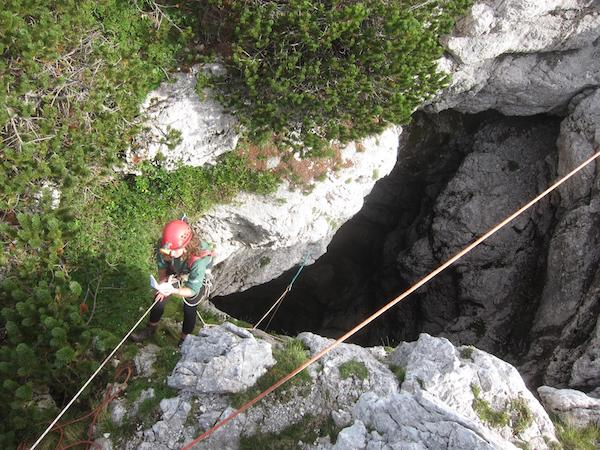
\includegraphics[width=\textwidth]{"images/2015/jack-m10-2015/frostm10_2015.jpg}}
		\caption{}
		\label{M102015}
	\end{subfigure}
	\hfill
	\begin{subfigure}{0.355\textwidth}
		\centering
		\frame{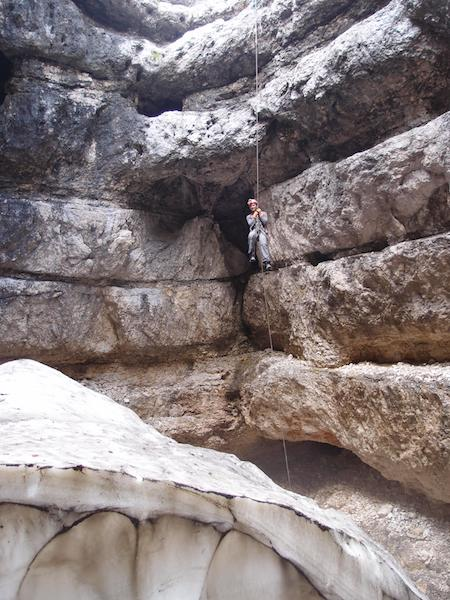
\includegraphics[width=\linewidth]{images/2015/jack-m10-2015/snowplugkan2015.jpg}}
		\caption{}\label{Kan2015}
	\end{subfigure}
	\caption{\emph{a}  On hot and dry summer days, snow is hauled from the M10 shakehole, located metres away from the Bivi --- Jarvist Frost \emph{b}  In summer, the cook shakeholes are choked with snowplugs of varying thickness --- Cecilia Kan}
\end{figure*}

Rhys was waiting impatiently, but seemed placated by my amusing story of testicular trauma. There is a broad, rock strewn ledge on the south side of M10, and this year the top of the snow was just level with this ledge. The snow plug was melted all the way round, and Rhys wriggled down under the overhanging rock to the space between the snow plug and the rock. It was a surreal place, cold and drippy, and the snow underneath kept threatening to give way.

With a bit of brute force we made it about a quarter of a turn clockwise round the snow plug, and found a crawling height passage going off normal to the rock. This quickly lead to a tight downclimb, which was inhabited by a beautiful ice stalactite. We squeeze past and into a small chamber below, where the lead died in a tight, immature rift. Pausing only to take a photo we headed back up and continued to traverse around the snow plug.

Another half a turn clockwise we found another passage heading off. The snow was very close to the top of the rock, but with some digging we opened up a passage and put some bolts in. Rhys slid down first - it was a slick icy slope at around 50 degrees. Two thirds of the way down was a passage on the left that lead to a chamber with a boulder strewn floor and a nice ice stalagmite. At the bottom of the slippery slope the cave ended - the water must go somewhere, but it’s frozen solid and the ice is as hard as the rock.

Who knows what wonders global warming will unleash in M10? It’s unlikely to go any time soon, but the siren song of a lead next to the bivvy will surely lure back more optimistic cavers for years to come.

\name{Jack Hare}

\begin{figure}[b!]
\checkoddpage \ifoddpage \forcerectofloat \else \forceversofloat \fi
\centering
\frame{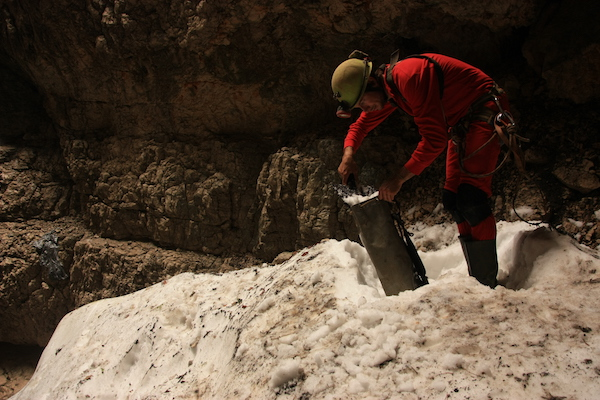
\includegraphics[width=\textwidth]{"images/2015/jack-m10-2015/gergely-m10_snow_shovelling.jpg}}
\caption{Shovelling snow at the bottom of M10 is hard work, but more important still is to establish clear communications between digger and hauling team, 20m directly above --- Gergely Ambrus}
\label{bottom of M10}
\end{figure}

